\documentclass[11pt]{article}
\usepackage{ucs}
\usepackage[utf8x]{inputenc}
\usepackage{changepage}
\usepackage{graphicx}
\usepackage{amsmath}
\usepackage{gensymb}
\usepackage{amssymb}
\usepackage{enumerate}
\usepackage{tabularx}
\usepackage{lipsum}
\usepackage{hyperref}
\usepackage{color}

\oddsidemargin 0.0in
\evensidemargin 0.0in
\textwidth 6.27in
\headheight 1.0in
\topmargin -0.1in
\headheight 0.0in
\headsep 0.0in
\textheight 9.0in

%\setlength\parindent{0pt}

\newenvironment{myenv}{\begin{adjustwidth}{0.4in}{0.4in}}{\end{adjustwidth}}
\renewcommand{\abstractname}{Anotācija}
\renewcommand\refname{Atsauces}



\newcounter{alphnum}
\newenvironment{alphlist}{\begin{list}{(\Alph{alphnum})}{\usecounter{alphnum}\setlength{\leftmargin}{2.5em}} \rm}{\end{list}}


%16.3-6
% 
% http://www.ccs.neu.edu/home/jaa/CS6800.11F/Homeworks/HW05.pdf


\makeatletter
\let\saved@bibitem\@bibitem
\makeatother

\usepackage{bibentry}
%\usepackage{hyperref}


\begin{document}

\thispagestyle{empty}

{\Large Lietišķie algoritmi \textendash{} 1. mājas darbs: Atrisinājumi}


{\footnotesize
\noindent
{\bf 1.uzdevums: Aritmētiskais kods (max 3 punkti).}
Dota ziņojumu kopa $S = \{ A,B,C,D \}$ ar attiecīgajām varbūtībām 
$\{ 0.2, 0.5, 0.2, 0.1 \}$.
\begin{enumerate}[(a)]
\item Parādīt, kā iegūt aritmētisko kodu $6$ ziņojumu virknei {\tt CBAABD} -- uzkonstruēt
tai atbilstošo intervālu $[l_6;l_6+s_6) \in [0;1]$ un atrast 
īsāko bitu virkni $d_1d_2\ldots{}d_{\ell}$ (visi $d_k \in \{ 0,1 \}$, 
kur pierakstot binārā pieraksta daļskaitlim $D = 0.d_1d_2\ldots{}d_{\ell}\ldots$ 
galā jebkuru turpinājumu ar cipariem $0$ vai $1$, iegūtais skaitlis $d+\varepsilon$ pieder
intervālam $[l_6;l_6+s_6)$.
\item Noteikt, kādu ziņojumu virkni alfabētā $S$ kodē skaitlis 
$D'' = 0.0011101011_2$.
\end{enumerate}
}

\noindent
{\bf (a)} Sākotnējais intervāls $[l_0;l_0+s_0] = [0;1]$. Uzrakstām tālākos 
sešus intervālus: 
$$\begin{array}{rcl}
I_1 & = & [0.70000,0.90000)\\
I_2 & = & [0.74000,0.84000)\\
I_3 & = & [0.74000,0.76000)\\
I_4 & = & [0.74000,0.74400)\\
I_5 & = & [0.74080,0.74280)\\
I_6 & = & [0.74260,0.74280)
\end{array}$$

Pēdējo intervālu $I_6$ kodē bitu virkne {\tt 1011111000100}, jo 
skaitlis ${\displaystyle 0.1011111000100_2 = \frac{6084}{2^{13}}}$
un 
$$\left[ \frac{6084}{2^{13}}; \frac{6085}{2^{13}} \right] \subseteq [0.74260,0.74280).$$
Kodiem garumā $13$ citus skaitļus (izņemot jau atrastos $6064/8192$ un $6065/8192$) izmantot nevar: 
intervāls pilnībā neietilps $I_6$.

{\em Piezīme:} Ja esat ņēmuši kodu, kurš garāks par $13$, tad
iespējami arī citi atrisinājumi. Tos neuzskatām par nepareiziem, ja vien 
Jūsu kodam atbilstošais intervāls pilnībā ietilpst intervālā $I_6$. 
Praksē lietojamie aritmētiskie kodi vai nu pievieno ziņojumu 
alfabētam EOF (faila beigu) ziņojumu vai nu arī kaut kur 
iekodē ziņojumu virknes garumu, lai 
atkodētājs zinātu, kur apstāties. 

Īpašs "pseido EOF" simbols mēdz būt aktuāls pat Hafmana koda vingrinājumos. 
Atšķirībā no bināriem skaitļiem, Hafmana prefiksu kodu virknē it kā ir redzams, kur 
vajag apstāties, bet praksē tas bieži nenostrādā, jo failam jāsatur vesels skaits baitu; 
pēc visu Hafmana kodavārdu izrakstīšanas var gadīties daži lieki biti, kurus negribam atkodēt. 
Plašāku diskusiju par "pseido EOF" sk. Stenfordas universitātes uzdotajā programmēšanas mājasdarbā:\\
\url{https://web.stanford.edu/class/archive/cs/cs106b/cs106b.1172/assn/huffman.html}. 


\noindent
{\bf (b)} Sākam ar intevālu 
$$[0.0011101011_2;0.0011101100_2) = [235/1024;236/1024) \approx [0.2294921875 0.2304687500).$$
Turpmākajos soļos noskaidrojam, kurā no ziņojumiem $\{ A,B,C,D \}$ atbilstošajiem intervāliem
($[0;0.2)$, $[0.2;0.7)$, $[0.7;0.9)$, $[0.9;1.0)$) šis intervāls ietilpst. 
Tiklīdz kā esam to atraduši, tad pierakstām atkodēto ziņojuma burtu un 
intervālu (kādu no $[0;0.2)$, $[0.2;0.7)$, $[0.7;0.9)$, $[0.9;1.0)$) ``izstiepjam'' tā, 
lai tas būtu garumā $[0;1]$. Pēc tam šo soli atkārto tikmēr, kamēr sākotnējais intervāls 
vairs nav viennozīmīgi ievietojams nevienā no tiem. Tad atkodēšana beidzas. 

\begin{itemize}
\item 1.solis: $I_1 = [0.2294921875 0.2304687500) \subseteq [0.2;0.7)$. Atkodēts {\tt B}.
\item 2.solis: No abiem $I_1$ galapunktiem atņem $0.2$ un dala ar $[0.2;0.7)$ garumu jeb $0.5$:\\
$I_2 = [0.058984375 0.060937500) \subseteq [0;0.2)$. Atkodēts {\tt A}.
\item 3.solis: No abiem $I_2$ galapunktiem atņem $0$ un dala ar $[0;0.2)$ garumu jeb $0.2$:\\
$I_3 = [0.294921875 0.304687500) \subseteq [0.2;0.7)$. Atkodēts {\tt B}.
\item 4.solis: Atņem $0.2$, dala ar $0.5$: $I_4 = [0.18984375 0.20937500)$. Intervāls vēl ir pietiekami 
īss, bet tas vairs nav viennozīmīgi atkodējams, jo šķeļas gan ar $[0;0.2)$, gan $[0.2;0.7)$. 
\end{itemize}

Atkodētais ziņojums ir ${\tt BAB}$. 

{\em Piezīme:} Praksē aritmētiskā koda atkodēšanas algoritms tiek pārcelts no peldošā punkta aritmētikas uz veselo skaitļu aritmētiku. 
Šajā gadījumā atkodē nevis visu intervālu, bet tikai tā kreiso galapunktu - piemēram, skaitli $235/1024$. 
Viens skaitlis allaž nonāks tieši vienā no $4$ apakšintervāliem un allaž varēs atkodēt.
Atkodēšanu turpina tikmēr, kamēr sasniegts "pseido EOF" simbols, par kuru rakstījām augstāk. 
Ja par "pseido EOF" uzskata ziņojumu {\tt D}, tad, atkodēšana rada citu atbildi ${\tt BABAD}$. 
Ja kādam bija šāda atbilde, tad arī tā atbilst citam aritmētiskā koda dialektam.\\
Ja atbilde ir pavisam cita (nevis {\tt BAB} vai {\tt BABAD}), tad Jūsu aprēķinos ir kļūda.




{\footnotesize 
\vspace{10ex}
\noindent
{\bf 2.uzdevums: Lempela-Ziva algoritms (max 4 punkti).}
\begin{enumerate}[(a)]
\item 
Ar LZ78 metodi nokodēt tekstu “abracadabra, abracadabra”.
\item Atkodēt ar LZ78 metodi nokodētu tekstu $a,b,c,d,2,5,a,6$, kur
$a$, $b$ un $c$ apzīmē atbilstošos burtus, bet skaitļi – vārdnīcas virkņu
numurus.
\item
Nokodēt (a) punkta tekstu “abracadabra, abracadabra” 
ar LZ77 metodi, kā logu lietojot visu nokodēto/atkodēto tekstu.
\end{enumerate}
}

\noindent
{\bf (a)} Teksts satur alfabēta simbolus $\mathtt{"a"}$, $\mathtt{"b"}$,
$\mathtt{"c"}$,$\mathtt{"d"}$,$\mathtt{"r"}$,$\mathtt{","}$,$\mathtt{"\;\;"}$, ieskaitot 
komatu un tukšumu. 

\begin{center}
\begin{tabular}{ |l|l|l|l|l| } \hline
Solis & $w$ & $k$ & Izvade & Pievieno vārdnīcai \\ \hline
1 & {\tt a} & {\tt "b"} & {\tt a} & {\tt ab} \\
2 & {\tt b} & {\tt "r"} & {\tt b} & {\tt br} \\ 
3 & {\tt r} & {\tt "a"} & {\tt r} & {\tt ra} \\ 
4 & {\tt a} & {\tt "c"} & {\tt a} & {\tt ac} \\ 
5 & {\tt c} & {\tt "a"} & {\tt c} & {\tt ca} \\ 
6 & {\tt a} & {\tt "d"} & {\tt a} & {\tt ad} \\ 
7 & {\tt d} & {\tt "a"} & {\tt d} & {\tt da} \\ 
8 & {\tt ab} & {\tt "r"} & {\tt ab} $\rightarrow$ 1 & {\tt abr} \\
9 & {\tt ra} & {\tt ","} & {\tt ra} $\rightarrow$ 3 & {\tt ra,} \\ 
10 & $\mathtt{","}$ & $\mathtt{"\;\;"}$ & $\mathtt{","}$ & $\mathtt{",\;\;"}$ \\
11 & $\mathtt{"\;\;"}$ & $\mathtt{a}$ & $\mathtt{"\;\;"}$ & $\mathtt{"\;\;a"}$ \\
12 & {\tt abr} & {\tt a} & {\tt abr} $\rightarrow$ 8 & {\tt abra}\\
13 & {\tt ac} & {\tt a} & {\tt ac} $\rightarrow$ 4 & {\tt aca}\\
14 & {\tt ad} & {\tt a} & {\tt ad} $\rightarrow$ 6 & {\tt ada}\\
15 & {\tt abra} & {\tt EOF} & {\tt abra} $\rightarrow$ 12 & $-$\\ \hline
\end{tabular}
\end{center}

Izvade: $\mathtt{a.b.r.a.c.a.d.1.3.","."\;\;".8.4.6.12}$.\\
{\em Piezīme.} Komatu un atstarpi likām pēdiņās un koda izvades atdalījām ar punktiem. 
(Reālā algoritma izvadē kodus atdala citādi - ar baitu robežām; tāpēc punkti un pēdiņas 
ir tikai pieraksta ērtība, nevis izvades sastāvdaļa.)
Atkarībā no tā, vai risinātājs tukšumu starp vārdiem pamanīja un uzskatīja par ziņojumu, 
iespējams arī cits, līdzīgs kodējums, par kuru vērtējums netiek samazināts.

\noindent
{\bf (b)}

\begin{center}
\begin{tabular}{ |l|l|l|l|l| } \hline
Solis & $w$ & $k$ & Izvade & Pievieno vārdnīcai \\ \hline
1 & {\tt a} & {\tt b} & {\tt a} & {\tt ab} \\
2 & {\tt b} & {\tt c} & {\tt b} & {\tt bc} \\ 
3 & {\tt c} & {\tt d} & {\tt c} & {\tt cd} \\ 
4 & {\tt d} & {\tt b} & {\tt d} & {\tt db} \\ 
5 & {\tt bc} & {\tt b} & {\tt bc} $\rightarrow$ 2 & {\tt bcb} \\ 
6 & {\tt bcb} & {\tt a} & {\tt bcb} $\rightarrow$ 5 & {\tt bcba} \\ 
7 & {\tt bcba} & {\tt EOF} & {\tt bcba} $\rightarrow$ 6 & $-$ \\ \hline
\end{tabular}
\end{center}

Atkodējums: $\mathtt{a.b.c.d.2.5.a.6}$ $\rightarrow$ $\mathtt{a.b.c.d.bc.bcb.a.bcba}$ $\rightarrow$ 
$\mathtt{abcdbcbcbabcba}$.



\noindent
{\bf (c)} Katrā LZ77 algoritma solī apzīmējam kursora stāvokli ar mazu pasvītrojumzīmi zem burta.
Garāko kopīgo apakšvirkni meklēšanas logā krāsojam sarkanu.
Iekavas, pēdiņas un semikoli mūsu ziņojumu alfabētā neietilpst, tie ir metasimboli, lai 
vieglāk uztvert LZ77 algoritma izvadi.

\noindent
$\underline{\mathtt{a}}\mathtt{bracadabra,\;\;abracadabra}$ \textendash{} izvade $(0;0;\mathtt{"a"})$\\
$\mathtt{a}\underline{\mathtt{b}}\mathtt{racadabra,\;\;abracadabra}$ \textendash{} izvade $(0;0;\mathtt{"b"})$\\
$\mathtt{ab}\underline{\mathtt{r}}\mathtt{acadabra,\;\;abracadabra}$ \textendash{} izvade $(0;0;\mathtt{"r"})$\\
$\mathtt{\textcolor{red}{a}br}\underline{\mathtt{a}}\mathtt{cadabra,\;\;abracadabra}$ \textendash{} izvade $(3;1;\mathtt{"c"})$\\
$\mathtt{\textcolor{red}{a}brac}\underline{\mathtt{a}}\mathtt{dabra,\;\;abracadabra}$ \textendash{} izvade $(5;1;\mathtt{"d"})^{\ast}$\\
$\mathtt{\textcolor{red}{abra}cad}\underline{\mathtt{a}}\mathtt{bra,\;\;abracadabra}$ \textendash{} izvade $(7;4;\mathtt{","})$\\
$\mathtt{abracadabra,}\underline{\;\;}\mathtt{abracadabra}$ \textendash{} izvade $(0;0;\mathtt{"\;\;"})$\\
$\mathtt{\textcolor{red}{abracadabra},\;\;}\underline{\mathtt{a}}\mathtt{bracadabra}$ \textendash{} izvade $(13;11;-)$\\


{\em Piezīme.} Dažreiz logā (jau nokodētajā teksta gabalā) atrodas vairāki visgarākie
apakšstringi; var izvēlēties starp diviem identiskiem apakšstringiem, kuru kopēt. 
Vēlāk kursā aplūkosim Bojera-Mūra garākās kopīgās apakšvirknes meklēšanas algoritmu; tas (līdzīgi 
citiem līdzīga veida algoritmiem) sāk virkņu salīdzināšanu no kreisās uz labo pusi. 
Tāpēc aplūkotajā piemērā, 5.solī izvadītais kods ir $(5,1,\mathtt{d})^{\ast}$
(kaut arī varēja rakstīt arī $(2,1,\mathtt{d})$ jeb skatīties atpakaļ nevis piecas pozīcijas, bet tikai divas). 
No atkodēšanas viedokļa nekādas atšķirības nav; tāpēc šajā piemērā (lai būtu konsekventi) rakstām 
pirmo atrasto pozīciju no kreisās puses. Bet par kļūdu neuzskatām arī jebkuru citu pozīciju, ja 
arī tā ir visgarākā. Diskusiju par šo apakšvirkņu meklēšanas metodēm sk.\ 
\url{https://bit.ly/2pD7m2Y} ({\em Longest-match String Searching for Ziv–Lempel Compression} by 
Timothy Bell, David Kulp). 


{\footnotesize
\vspace{10ex}
\noindent
{\bf 3.uzdevums: Berouza-Vīlera transformācija (max 3 punkti).}
\begin{enumerate}[(a)]
\item Kāds ir rezultāts (transformētā simbolu virkne un 
sākotnējās virknes pozīcija), lietojot 
Berouza-Vīlera transformāciju 
$14$ simbolu virknei {\tt alusariirasula}?
\item Kāds ir iepriekšējā piemērā iegūtās transformētās simbolu virknes pieraksts,
izmantojot Move-to-Front kodēšanu?
\item Pēc BW transformācijas pielietošanas tika iegūta simbolu virkne 
{\tt mmmrvvauuuiibbbri}. Kāda bija simbolu virkne pirms 
transformācijas (ņemot 4.\ virkni
no atjaunotās tabulas)?
\end{enumerate}
}


\noindent
{\bf (a)} Ja lietojam to Berouza-Vīlera transformāciju, kāda tā aprakstīta 
Vikipēdijā: \url{https://en.wikipedia.org/wiki/Burrows%E2%80%93Wheeler_transform} 
\textendash piemērā ar vārdu {\tt \^{}BANANA|}, tad 
izrakstām visas $14$ cikliskās permutācijas vārdam {\tt alusariirasula}
($0,1,2,\ldots,13$ burtus no šī vārda beigām pārceļam uz tā sākumu). Pēc tam 
šīs permutācijas (rindiņas zemāk attēlotajā tabulā) sakārtojam leksikogrāfiski: 
vienkārši sakot, pēc alfabēta: Vispirms izrakstām visas permutācijas, kam
pirmais burts ir "a" (tās sašķiro pēc 2.burta; ja arī tas sakrīt, pēc 3.burta, utt.). 

Pēc tam ievērojam, ka pēdējā tabulas kolonnā rakstīts  {\tt lasrriuaiauasl}. 
Mūsu sākotnējās virknes {\tt alusariirasula} indekss ir $1$ (šī 
virkne redzama tabulas 2.rindiņā), bet indeksus sāk
numurēt, sākot no $0$: 2.rindiņas indekss tāpēc ir $1$. 

\begin{verbatim}
aalusariirasul
alusariirasula
ariirasulaalus
asulaalusariir
iirasulaalusar
irasulaalusari
laalusariirasu
lusariirasulaa
rasulaalusarii
riirasulaalusa
sariirasulaalu
sulaalusariira
ulaalusariiras
usariirasulaal
\end{verbatim}

\noindent
{\bf (b)} Kāds kods rodas no Move-to-Front, ja to lieto 
virknei {\tt lasrriuaiauasl}, kur alfabētiskais
sakārtojums ir $\mathtt{a}<\mathtt{i}<\mathtt{l}<\mathtt{r}<\mathtt{s}<\mathtt{u}$, kur burtu indeksus sāk skaitīt, 
sākot no 0.indeksa?

\noindent
Rakstām tabulu, kurai augšējā rindiņā ir kodējamais vārds, bet
alfabētus rakstām vertikāli uz leju:\\
\begin{tabular}{c|cccccccccccccc}
Alfabēts$\downarrow$ & l & a & s & r & r & i & u & a & i & a & u & a & s & l \\ \hline
a                    & l & a & s & r & r & i & u & a & i & a & u & a & s & l \\ 
i                    & a & l & a & s & s & r & i & u & a & i & a & u & a & s \\ 
l                    & i & i & l & a & a & s & r & i & u & u & i & i & u & a \\ 
r                    & r & r & i & l & l & a & s & r & r & r & r & r & i & u \\ 
s                    & s & s & r & i & i & l & a & s & s & s & s & s & r & i \\ 
u                    & u & u & u & u & u & u & l & l & l & l & l & l & l & r \\ \hline
Izeja:               & 2 & 1 & 4 & 4 & 0 & 4 & 5 & 4 & 2 & 1 & 2 & 1 & 4 & 6 
\end{tabular}


\noindent
{\bf (a) un (b) citam Berouza-Vīlera transformācijas variantam:}\\
Ja izmantojam Guy E.Blelloch grāmatu "Introduction to Data Compression", tad
Berouza-Vīlera transformāciju iegūst, sakārtojot cikliskās permutācijas
leksikogrāfiski pēc priekšpēdējā burta, ja sakrīt, tad pēc priekšpriešpēdējā, utt. 
Transformācijas rezultāts arī šajā gadījumā ir pēdējā kolonna. 

\begin{verbatim}
usariirasulaal
lusariirasulaa
ulaalusariiras
iirasulaalusar
asulaalusariir
rasulaalusarii
sariirasulaalu
alusariirasula
irasulaalusari
sulaalusariira
laalusariirasu
riirasulaalusa
aalusariirasul
ariirasulaalus
\end{verbatim}

Berouza-Vīlera transformācijas rezultāts ir pēdējā kolonna: {\tt lasrriuaiauals}. 
Tas ir cits vārds nekā {\tt lasrriuaiauasl} (pēdējie $2$ burti ir pretējā secībā). 
Arī Move-to-Front kods izskatās citādi: 
$$214404542121\textcolor{red}{66}\;\;\text{nevis}\;\;214404542121\textcolor{red}{46}$$
kā iepriekšējā variantā.





{\footnotesize
\vspace{10ex}
\noindent
{\bf 4.uzdevums: I-iespēja (max 10 punkti).} 
Pieņemsim, ka ziņojumu kopai $S = \{ x_1, x_2, \ldots, x_n \}$ ar 
izveidots optimāls prefiksu kodējums. Šis kodējums jāpārraida,
izmantojot minimālu bitu skaitu.\\
Pierādīt vai apgāzt šādu 
apgalvojumu: Jebkuru optimālu prefiksu 
kodējumu šai $n$ ziņojumu kopai var nosūtīt, izmantojot ne vairāk kā 
${\displaystyle 2n - 1 + n \left\lceil log_2 n \right\rceil}$ bitus. 
Šeit $\lceil x \rceil$ apzīmē noapaļošanu uz augšu jeb 
mazāko veselo skaitli, kas nav mazāks par $x$.
Piemēram $\lceil 17 \rceil = 17$ un $\lceil 3.14 \rceil = 4$.\\
{\em Ieteikums.} Izmantojot $2n-1$ bitus, var attēlot kodējumu koka 
virsotņu apstaigāšanas secību.
}

Pamatosim, ka prefiksu koku var nosūtīt, izmantojot ne vairāk kā
${\displaystyle 2n - 1 + n \left\lceil log_2 n \right\rceil}$ bitus.\\

Tad, ja būtu jānosūta vienkārši $n$ alfabēta simbolu permutācija (viens no $n!$ 
iespējamajiem šo ziņojumu izkārtojumiem, kurā katrs ziņojums parādās tieši vienu reizi), 
tad pietiktu ar $n \left\lceil log_2 n \right\rceil$ bitiem. Teiksim, 
$3$ simbolu permutācijai (kādai no virknēm $\mathtt{ABC}$, 
$\mathtt{ACB}$, $\mathtt{BAC}$, $\mathtt{BCA}$, $\mathtt{CAB}$ vai $\mathtt{CBA}$)
iztērējas $3 \cdot 2 = 6$ biti, jo katru no trim burtiem var uzrakstīt 
ar $2$ bitu virknīti. 

Tomēr jāatceras, ka mūsu mērķis ir nosūtīt nevis simbolu permutāciju, bet 
bināru koku, kurā šie simboli parādās kā "koka lapas" (balti aplīši zīmējumā). 

\begin{center}
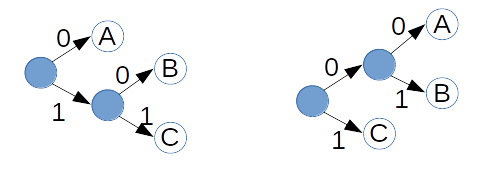
\includegraphics[width=3in]{prefix-trees.png}\\
{\em Zīmējums: 2 prefiksu koki ziņojumu alfabētam $S = \{ A,B,C\}$.}
\end{center}

Lai šos kokus varētu atšķirt, var izmantot bināro operatoru $\ast$ un iekavas. Piemēram: 
$$\mathtt{(A}\ast\mathtt{(B}\ast\mathtt{C))}\;\;\text{un}\;\;\mathtt{((A}\ast\mathtt{B)}\ast\mathtt{C)}.$$
Šajā sintaksē simbols $\ast$ apzīmē divu bināru koku salīmēšanas darbību. 
Ir vēl taupīgāks pieraksta veids \textendash{} "apgrieztais poļu pieraksts"
({\em Reverse Polish Notation}), kurā 
$\mathtt{(A}\ast\mathtt{B)}$ aizstāj ar $\mathtt{AB}\ast$. Šajā sintaksē iekavas nav vajadzīgas, 
bet koku vienalga var atjaunot. 
Zīmējumā attēlotie prefiksu koki apgrieztajā poļu pierakstā būs šādi:\\
$\mathtt{ABC}\ast\ast$ un $\mathtt{AB}\ast\mathtt{C}\ast$

Vispārīgajā gadījumā, lai izveidotu šādu poļu pieraksta izteiksmi no $n$ simboliem, 
jāpieraksta šie simboli kaut kādā secībā un vēl $n-1$ zvaigznītes (binārā kokā 
ar $n$ lapām būs tieši $n-1$ iekšējas virsotnes \textendash{} lai no $n$ gabaliņiem izveidotu 
vienu koku, jālīmē kopā tieši $n-1$ reizes). 
Tā kā zvaigznīšu ir daudz, tās kodēsim vienkārši ar
bitu "1", bet katram ziņojumu alfabēta $S$ simbolam $x_i$ rakstīsim priekšā 
bitu "0".

{\bf Kodējuma piemēri:} Aplūkosim jau minēto
prefiksu koku {\tt (A$\ast$(B$\ast$C))}, kurš zīmējumā redzams pa kreisi: Tajā simbolu {\tt A} kodē ar 
virknīti "0", simbolu {\tt B} kodē ar "10", bet simbolu {\tt C} kodē ar "11".

Šī prefiksu koka apgrieztais poļu pieraksts ir $\mathtt{ABC}\ast\ast$. 
Tā kā saņēmējs vēl nezina, kā tiks kodēti ziņojumu alfabēta simboli,
tad kodējam tos vienkārši pēc kārtas ar vienāda garuma 
virknēm, kas visas sākas ar bitu "0". 
Simbola {\tt A} fiksētā garuma kods (prefiksu koka nosūtīšanai, 
nevis Hafmana kodēšanai ar mainīgā garuma kodu) būs 
virkne "000", {\tt B} kods būs virkne "001", 
{\tt C} kods būs "010". Tā kā $n=3$ nav divnieka pakāpe, tad virkne "011" paliek neizmantota. 

Pierakstu $\mathtt{ABC}\ast\ast$ tātad kodē virkne "000 001 010 1 1" (atkodēšanai atstarpes nevajag).\\
Savukārt citu bināro koku $\mathtt{AB}\ast\mathtt{C}\ast$, kas zīmējumā redzams pa labi, 
apzīmē virkne "000 001 1 010 1".

Patvaļīgam $n$ prefiksu koka kodējums sastāv no $n$ dažādiem ziņojuma simboliem \textendash{} katru 
no tiem kodē garumā $\left\lceil \log_2 n \right\rceil + 1$ biti. Vajadzīgas arī $n-1$ 
zvaigznītes. Katru no tiem kodē ar $1$ bitu. Kopīgais bitu skaits:
$$n\cdot\left( \left\lceil \log_2 n \right\rceil + 1 \right) + 
(n-1)\cdot{}1 = 2n-1 + n \left\lceil \log_2 n \right\rceil.$$
$\blacksquare$


\end{document}



